\pagestyle{plain}
\pagenumbering{arabic}
\setcounter{page}{2}

\refsection

%\clearpage
%\thispagestyle{empty}

%\vfill

%\begin{center}
%[Место для распечатки отчета Антиплагиата]
%\end{center}

%\newpage
%\thispagestyle{empty}

%\vfill

%\begin{center}
%[Место для распечатки отчета Антиплагиата]
%\end{center}

\clearpage

\chapter*{Реферат}
\thispagestyle{plain}

Общий объем основного текста, без учета приложений — \pageref{end_of_main_text} страниц, с учетом приложений — 61. Количество использованных источников — 16. Количество приложений — 2.

\noindent \uppercase{лямбда-исчисление, бета‑редукция, абстрактная машина, F\#, FParsec}

Целью данной работы является разработка расширяемой библиотеки на платформе .NET и языке F\# для синтаксического анализа и пошаговой бета‑редукции лямбда‑термов с возможностью конфигурирования стратегий редукции и операторов.

В первой главе проводится обзор литературы по аппликативным методикам организации вычислений, сравнительный анализ стратегий бета‑редукции и возможностей платформы .NET для реализации асинхронных и параллельных вычислений.

Во второй главе описывается используемая модель расширяемой аппликативной вычислительной среды, выбор и формализация стратегий редукции, разработка структур данных и метаданных для представления термов, а также выбор синтаксиса учебного языка.

В третьей главе приводятся результаты проектирования: архитектура системы, API абстрактной машины бета‑редуктора и синтаксических анализаторов, описаны их интерфейсы и взаимодействие компонентов.

В четвертой главе изложена реализация и экспериментальная проверка: ключевые фрагменты кода парсера и машины, описание тестовых примеров, результаты тестирования и сравнение с существующими аналогами.

В приложении \ref{app-format} представлены основные структуры разработанного модуля.

В приложении \ref{app-format1} представлены тесты основного модуля.



\clearpage

\tableofcontents{}

\clearpage

\chapter*{Введение}
\label{sec:afterwords}
\addcontentsline{toc}{chapter}{Введение}

Введение всегда содержит краткую характеристику работы по следующим аспектам:

\begin{itemize}
	\item актуальность:
	\begin{itemize}
		\item кто и почему в настоящее время интересуется данной проблематикой (в т.ч. для решения каких задач могут быть полезны исслелования в данной области),
		\item краткая история вопроса (в формате год-фамилия-что сделал),
		\item нерешенные вопросы/проблемы;
	\end{itemize}
	\item новизна работы (что нового привносится данной работой);
	\item оригинальная суть исследования;
	\item содержание по главам (по одному абзацу на главу).
\end{itemize}

Общий объем введения должен не превышать 1,5 страниц (для ПЗ к УИРам может быть чуть меньше).

%%% Local Variables:
%%% TeX-engine: xetex
%%% eval: (setq-local TeX-master (concat "../" (seq-find (-cut string-match ".*-3-pz\.tex$" <>) (directory-files ".."))))
%%% End:


\clearpage

\chapter{Анализ проблематики программной реализации Бета-редуктора}
\label{chapter1}

\section{Изучение и анализ литературы по аппликативным методикам организации вычислений}

Лямбда‑исчисление было предложено А. Чёрчем в 1932 году как формализм для исследования функций и рекурсии \cite{ChurchRosser}. Основные объекты в лямбда‑исчислении, называемые \emph{лямбда‑термами}, строятся по трём правилам: введение \emph{переменной}, \emph{абстракции} и \emph{аппликации} — например, если $x$ и $y$ — переменные, то $\lambda x.\,x\,y$ является термом .  

Операция \emph{бета‑редукции} формализует применение функции к аргументу. Формально, для терма вида $(\lambda x.\,M)\,N$ результатом одного шага бета‑редукции является терм $M[x := N]$, где $M[x := N]$ обозначает подстановку $N$ вместо всех свободных вхождений $x$ в $M$ .  

Ключевым свойством бета‑редукции является \emph{конфлюэнтность} (теорема Чёрча — Россера): если терм $M$ может быть приведён двумя разными способами к $N_1$ и $N_2$, то существует терм $P$, в который $N_1$ и $N_2$ могут быть дополнительно редуцированы — это гарантирует однозначность нормальной формы независимо от выбранной стратегии редукции .  
\label{sec:theory-beta}
\subsection{Определение лямбда‑термов}
Лямбда‑термы строятся по трём правилам \cite{Barendregt1984}:
\begin{enumerate}
  \item Любая переменная \(x\) является термом.
  \item Если \(M\) и \(N\) — термы, то их аппликация \((M\ N)\) также является термом.
  \item Если \(x\) — переменная, а \(M\) — терм, то \(\lambda x.\,M\) (лямбда‑абстракция) является термом.
\end{enumerate}
Обозначим множество всех лямбда‑термов как \(\Lambda\).  

\subsection{Свободные и связанные переменные; альфа‑конверсия}
В терме \(\lambda x.\,M\) все вхождения \(x\) в \(M\) считаются \emph{связанными}, остальные переменные называются \emph{свободными}. Обозначим множества свободных и связанных переменных терма \(M\) как \(\mathrm{FV}(M)\) и \(\mathrm{BV}(M)\) соответственно \cite{HindleySeldin2008}.  

Для предотвращения конфликтов при подстановке вводят операцию \emph{альфа‑конверсии}: 
\[
  \lambda x.\,M \;\equiv_\alpha\;\lambda y.\,(M[x\mapsto y]),
\]
где \(y\) не входит в \(\mathrm{FV}(M)\). Альфа‑конверсия сохраняет семантику терма, меняя только связанные имена переменных.

\subsection{Определение бета‑редукции}
Бета‑редукция — это операция применения функции к аргументу:
\[
  (\lambda x.\,M)\;N \;\to_\beta\; M[x := N],
\]
где \(M[x := N]\) обозначает \emph{подстановку} \(N\) вместо свободных вхождений \(x\) в \(M\) \cite{Pierce2002}.  

Подстановка \(M[x:=N]\) определяется рекурсивно:
\[
  \begin{aligned}
    x[x:=N] &= N,\\
    y[x:=N] &= y,\quad y\neq x,\\
    (P\ Q)[x:=N] &= (P[x:=N])\;(Q[x:=N]),\\
    (\lambda y.\,P)[x:=N] &=
      \begin{cases}
        \lambda y.\,P[x:=N], & y\notin\mathrm{FV}(N),\\
        \lambda z.\,(P[y:=z])[x:=N], & y\in\mathrm{FV}(N),\; z\notin\mathrm{FV}(P)\cup\mathrm{FV}(N).
      \end{cases}
  \end{aligned}
\]
Второй случай лямбда‑абстракции требует переименования (альфа‑конверсии), если \(y\) встречается в \(N\), чтобы избежать захвата свободных переменных.

\subsection{Нормальная форма и стратегия редукции}
Терм \(M\) называется \emph{бета‑нормальным}, если в нём нет подтермов вида \((\lambda x.\,P)\,Q\). Нормальная форма терма, если она существует, единственна (до альфа‑конверсии) благодаря конфлюэнтности бета‑редукции \cite{ChurchRosser}.  

Различают две классические стратегии применения шагов бета‑редукции \cite{Plotkin1975}:
\begin{itemize}
  \item \textbf{Нормальный порядок} (normal order): в каждый момент редуцируется самый внешний левый редекс. Эта стратегия гарантирует достижение нормальной формы, если та существует.
  \item \textbf{Аппликативный порядок} (applicative order): сначала редуцируются аргументы, затем само применение. Может не завершиться, даже если нормальная форма существует.
\end{itemize}
Аппликативные методики организации вычислений представляют собой важный раздел теории вычислений, восходящий к работам Чёрча и Карри. В современной литературе (например, \cite{Wolfengagen2004}) выделяют несколько ключевых подходов:

\begin{itemize}
    \item \textbf{Аппликативные порядки вычислений} - стратегии определения момента вычисления аргументов функций
    \item \textbf{Графовые модели вычислений} - представление программ в виде направленных ациклических графов
    \item \textbf{Абстрактные вычислительные машины} - формальные модели для реализации стратегий вычислений
\end{itemize}

\subsection{Аппликативные вычислительные системы}
В работе В.Э. Вольфенгагена \cite{Wolfengagen2004} подробно рассматриваются различные аппликативные вычислительные системы, что стало основным материалом в аналитической части учебно исследовательской работы. Вячеслав Эрнстович предлагает классификацию, включающую:

\begin{itemize}
  \item Формализацию термов первого и высшего порядков
  \item Построение абстрактных машин через синтаксические правила редукции
  \item Анализ производительности различных моделей редукции
  \item Стратегии управления контекстом (environment, stack) при бета-редукции
\end{itemize}

Эти теоретические основы легли в основу:
\begin{enumerate}
  \item выбора представления термов в виде атомиков и композитов
  \item реализации внутреннего буфера окружения для эффективной подстановки
\end{enumerate}

\section{Сравнительный анализ стратегий редукции лямбда-выражений}

\subsection{AST vs.\ графовое представление термов}
Традиционный подход к бета‑редукции основан на работе с абстрактным синтаксическим деревом (AST): каждый шаг редукции создаёт новый AST, в котором подтермы копируются при подстановке — это просто в реализации, но порождает значительные издержки по памяти и времени на копирование одинаковых поддеревьев \cite{Pierce2002}\cite{HindleySeldin2008}.  

Альтернативно, в \emph{графовой редукции} (graph reduction) используют ориентированный ациклический граф (DAG), где общий подтерм хранится единожды и на него указывают несколько ссылок. При редукции заменяются лишь указатели, что позволяет избежать многократного копирования и реализовать мемоизацию (sharing) для ленивых стратегий — основа реализации ленивого Haskell в GHC на механизме STG \cite{PeytonJones1992}\cite{Barendregt1993}.  

\subsection{Модели управления окружением и стеком}
Классическая \textsc{SECD}‑машина Ландина разделяет состояние на четыре регистра: стек (S), окружение (E), управляющую последовательность (C) и дамп (D). При приведении аппликации элементы попарно обрабатываются с сохранением контекста в дампе — подход наглядный, но сравнительно громоздкий в реализации \cite{Landin1964}\cite{Felleisen1987}.  

\textsc{CEK}‑машина упрощает SECD: объединяет дамп и стек продолжений в одну структуру Kontinuation (K), сохраняя при этом разделение Control (C) и Environment (E). Она особенно хорошо подходит для call‑by‑value семантики и теоретических доказательств корректности вычислений \cite{Felleisen1987}\cite{Plotkin1975}.  

Машина Кривина оптимизирована для call‑by‑name: она хранит окружение в виде ассоциаций переменных с замыканиями и использует стек аргументов без дополнительного дампинга, что даёт минимальные накладные расходы при редукции \cite{Krivine2007}\cite{Barendregt1984}.  

\subsection{Оптимизации и стратегии редукции}
\emph{Call‑by‑need} (ленивая) стратегия сочетает normal order с мемоизацией: первый раз при обращении к редексу происходит редукция и результат сохраняется, при последующих обращениях переиспользуется — это устраняет повторные вычисления, сохраняя гарантию достижения нормальной формы \cite{Barendregt1993}\cite{Wadler1987}.  

Для строгих языков (call‑by‑value) разработаны оптимизации вроде \emph{tail‑recursion elimination} и \emph{deforestation}, которые устраняют промежуточные структуры при последовательных аппликациях, что критично для производительности в реализованных на C и JVM интерпретаторах \cite{PeytonJones1992}\cite{Wadler1990}.  


\section{Сравнительный анализ алгоритмов Бета‑Редукций}
\label{sec:comparison-beta}


\begin{table}[h]
\caption{Сравнительный анализ стратегий бета‑редукции}
\label{tbl:cmp-strategies}
\centering
\footnotesize
\begin{tabular}{|c|l|c|c|c|}
\hline
№ & Стратегия & Порядок & НФ & Эффективность \\
\hline
1 & Normal & Слева наружу & Да, если есть & Низкая \\
2 & CBN & Наружу, без замены & Не гарантирована & Высокая \\
3 & CBV & Слева внутрь & Быстрая, но не всегда & Высокая \\
4 & Lazy & С мемоизацией & Как Normal & Наилучшая \\
5 & Full & Любой редекс & Да, теоретически & Непрактична \\
\hline
\end{tabular}
\end{table}

\medskip

\noindent
Из таблицы \ref{tbl:cmp-strategies} видно, что наивные AST‑алгоритмы просты в реализации, но имеют большие накладные расходы по памяти и не всегда гарантируют достижение нормальной формы (для applicative order). Абстрактные машины CEK и Krivine оптимизированы для своих стратегий: первая эффективна для strict‑языков, вторая — для ленивых. Graph‑редукция сочетает гарантии нормальной формы (call‑by‑need) с малым расходом памяти благодаря разделению поддеревьев.


\section{Изучение возможностей платформы .NET для реализации асинхронных вычислений}
\label{sec:dotnet-async}

В процессе подготовки к проекту было проведено исследование программных решений, содержащих реализацию бета‑редукции. Основу анализа составили интерпретаторы, proof assistant’ы и экспериментальные среды, в которых реализована одна или несколько стратегий редукции. В ходе исследования учитывались открытые исходные коды, спецификации и научные публикации, подтверждающие архитектурные особенности инструментов.  

На основе результатов анализа была составлена сравнительная таблица. Особое внимание уделено выбору языков реализации, стратегии редукции, сложности расширения и целевого применения инструментов.

\begin{table}[h]
\caption{Сравнение программных средств для бета‑редукции}
\label{tbl:cmp-tools-beta}
\centering
\small
\begin{tabular}{|c|l|l|l|l|}
\hline
№ & Инструмент & Язык & Стратегия & Особенности \\
\hline
1 & Mace & F\# (.NET) & Normal, Full & Модульная архитектура, AST \\
2 & GHCi & Haskell & Call‑by‑need & STG‑машина, граф‑редукция \\
3 & Coq & OCaml & Call‑by‑value & Формализация λ-исчисления \\
4 & Agda & Haskell & Normal/CBV & Зависимая типизация \\
5 & PAKCS & Java & CBV/CBN & Функц.-логическая семантика \\
6 & LC Playground & JS/Web & Normal/App & Визуализация, браузерный \\
\hline
\end{tabular}
\end{table}
Платформа .NET и язык F\# предоставляют развитую инфраструктуру для как функциональных, так и асинхронных и параллельных вычислений.

\subsection{Функциональные возможности F\#}
\begin{itemize}
  \item \textbf{Система типов и сопоставление с образцом.} F\# поддерживает параметрические и алгебраические типы, а также мощное сопоставление с образцом, что упрощает представление и обработку лямбда‑термов и их подструктур \cite{Syme2015}.
  \item \textbf{Отложенные вычисления.} Механизм \texttt{lazy} и тип \texttt{Lazy<'T>} позволяют реализовать семантику Call‑by‑Need без сторонних библиотек \cite{Syme2015}.
  \item \textbf{Функциональные конструкции.} Встроенные функции высшего порядка, каррирование и композиция облегчают определение операций редукции как чистых функций \cite{Syme2015}.
\end{itemize}

\subsection{Асинхронные и параллельные вычисления}
\begin{itemize}
  \item \textbf{Task-based Asynchronous Pattern (TAP).} Поддержка \texttt{async/await} в C\# и F\# позволяет описывать асинхронные алгоритмы в линейном синтаксисе, компилируя их в эффективные конечные автоматы \cite{Richter2013}.
  \item \textbf{Параллельные коллекции.} PLINQ и \texttt{Parallel.ForEach} из пространства имён \texttt{System.Threading.Tasks} обеспечивают простой распараллеливание обработки больших наборов данных \cite{Duffy2008}.
  \item \textbf{Агенты (MailboxProcessor).} Фреймворк акторов в F\# через \texttt{MailboxProcessor<'Msg>} позволяет строить неблокирующие конвейерные и реактивные модели вычислений без явных примитивов синхронизации \cite{Syme2015}.
\end{itemize}

\subsection{Преимущества выбора платформы .NET}
\begin{enumerate}
  \item \textbf{Интеграция с CLR.} Возможность смешанного использования модулей на F\#, C\# и других языках .NET упрощает рефакторинг и расширение кодовой базы \cite{Richter2013}.
  \item \textbf{Производительность.} JIT‑компиляция и оптимизации многопоточности обеспечивают высокую скорость выполнения как синхронного, так и асинхронного кода \cite{Richter2013,Duffy2008}.
  \item \textbf{Экосистема и инструментарий.} Богатый набор библиотек NuGet, поддержка DevOps и облачных сервисов Azure позволяют быстро разрабатывать и деплоить распределённые приложения.
\end{enumerate}

\section{Выводы}

На основе проведённого анализа литературы и существующих программных решений можно сформулировать следующие ключевые выводы:

\begin{enumerate}
  \item Бета-редукция, являясь центральной операцией в лямбда-исчислении, обладает свойством конфлюэнтности, что позволяет добиться единственной нормальной формы независимо от стратегии редукции, при условии её существования.
  
  \item Различные стратегии редукции (normal order, call-by-name, call-by-value, lazy, full) обладают разной эффективностью и применимостью. Среди них наиболее практически значимой является \emph{ленивая стратегия (call-by-need)}, сочетающая мемоизацию и гарантии достижения нормальной формы.
  
  \item Представление термов в виде AST удобно, но неэффективно с точки зрения производительности и использования памяти. Графовое представление (DAG) позволяет существенно оптимизировать вычисления за счёт совместного использования поддеревьев и реализации sharing.
  
  \item Абстрактные вычислительные машины (SECD, CEK, Krivine) демонстрируют различные подходы к управлению окружением и продолжениями. Машина Кривина показывает высокую эффективность для ленивых стратегий, а CEK — для строгих.
  
  \item Среди исследованных программных решений платформа .NET (и язык F\#) показали высокую пригодность для реализации бета-редукции. F\# предлагает выразительные функциональные конструкции и развитую поддержку асинхронности, а CLR обеспечивает производительность и масштабируемость.
  
  \item Использование агентов (MailboxProcessor), отложенных вычислений (\texttt{Lazy}), а также параллельных коллекций делает .NET особенно подходящей для построения гибких и расширяемых интерпретаторов лямбда-исчисления с различными стратегиями редукции.
  
  \item Исследование существующих инструментов (Mace, GHCi, Coq, Agda и др.) показало отсутствие универсального решения. Большинство систем оптимизированы под одну стратегию и трудны к адаптации, что подчёркивает необходимость проектирования собственного расширяемого интерпретатора.
\end{enumerate}


\section{Постановка задачи}

Целью работы является разработка расширяемой системы для учебного изучения аппликативных вычислений, основанной на пошаговой редукции лямбда-выражений, с гибко настраиваемым синтаксисом, поддержкой различных стратегий редукции и использованием возможностей платформы .NET.

Для достижения поставленной цели необходимо решить следующие задачи:

\begin{enumerate}
  \item \textbf{Разработка теоретической модели:}
  \begin{itemize}
    \item Определить математическую основу системы, используя расширяемую предструктуру как модель аппликативной вычислительной среды.
    \item Выбрать и формализовать стратегии редукции, адаптированные под особенности модели и обеспечивающие поддержку пошагового вычисления.
    \item Разработать структуры данных и метаданные для описания термов, абстракций, аппликаций, редукций, атомиков и специальных комбинаторов.
    \item Выбрать и описать синтаксис учебного языка, обеспечивающий удобное представление выражений и читаемость для пользователей.
  \end{itemize}

  \item \textbf{Проектирование программной архитектуры:}
  \begin{itemize}
    \item Построить открытую архитектуру системы, основанную на контрактной модели, в которой основные компоненты реализуют общие интерфейсы.
    \item Спроектировать API для синтаксических анализаторов, обеспечивающий поддержку настраиваемого синтаксиса и расширяемости через конфигурации и колбэки.
    \item Описать взаимодействие компонентов с использованием диаграмм UML.
  \end{itemize}

  \item \textbf{Технологическая реализация и тестирование:}
  \begin{itemize}
    \item Реализовать абстрактную машину редукции и синтаксические анализаторы на F\#, с использованием современных средств платформы .NET.
    \item Разработать тестовые выражения и автоматизированные тесты для проверки корректности парсинга, редукции и ошибок.
    \item Оценить производительность реализации на различных примерах, в том числе с учётом глубины редукции, объема памяти и времени исполнения.
  \end{itemize}
\end{enumerate}

Выбор технологического стека (F\#, .NET) обусловлен необходимостью поддержки функционального стиля, типизации, высокоуровневой абстракции и наличием развитой инфраструктуры для построения расширяемых систем. Результаты работы планируется интегрировать в существующую платформу для изучения вычислительных моделей, расширив её функциональность и применимость в учебных целях.


\clearpage

\chapter{Теоретическая часть}
\section{Использованная модель аппликативной вычислительной среды на основе расширенной предструктуры}
\label{sec:extended-prestructure}

Разрабатываемый Бета-редуктор опирается на формальную модель \textit{аппликативной вычислительной среды} с \emph{расширенной предструктурой}.
Данная модель предоставляет основу для представления термов, механизмов аппликации и редукции \cite{Roslovtsev2011}.

\subsection*{Модель среды}
Предструктура АСВ (аппликативной среды вычислений) представляет собой пару 
$$ (D, F), $$
где $D$ --- это наборы исходных объектов, а $F$ --- набор термообразующих функций.

Расширяемость предструктуры реализована за счет возможности пополнять множества $D$ и $F$
в зависимости от конкретной среды.
В частности такой подход предоставляет преимущество в формализации и сравнительном анализе нескольких сред.

В разработанной системе роль исходных объектов играют атомики --- объекты, реализующие интерфейс \texttt{IAtomic};
роль термообразующих функций --- объекты, реализующие интерфейс \texttt{ITFF}.
Использование механизма полиморфизма через интерфейсы и позволяет реализовать упомянутую расширяемость предструктуры АСВ
(без модификации ядра системы).

\section{Выбор реализуемых стратегий редукции, моделирование пошагового процесса редукции с учётом особенностей модели расширяемой аппликативной среды}
\label{sec:reduction-strategies}

В предлагаемой расширяемой аппликативной среде был сделан упор на описанные Вольфенгагеном подходы в главах 5 и 6 его работы \cite{Wolfengagen2004}, где рассматриваются $\lambda$-исчисление, подстановка и основные понятия редукции.

\subsection{Выбор стратегий редукции}

Для реализации в среде были выбраны следующие стратегии:

\begin{itemize}
  \item \textbf{Нормальный порядок (Normal Order)} — всегда редуцируется самый левый внешний редекс. Гарантирует достижение нормальной формы \cite[§5.2.4, §5.4.2]{Wolfengagen2004}.
  \item \textbf{Аппликативный порядок (Applicative Order)} — сначала редуцируются аргументы, затем функция. Подробно обсуждается в разделе 6.6 подстановки и комбинаторов \cite[§6.6]{Wolfengagen2004}.
  \item \textbf{Call-by-Need (ленивая стратегия)} — нормальный порядок с мемоизацией, минимизирующей повторные вычисления, концептуально основана на идеях графовой редукции и call-by-need, упомянутых Вольфенгагеном в главе 12 \cite{Wolfengagen2004}.
\end{itemize}

\subsection{Пошаговое моделирование редукции}

Модель пошагового редукционного процесса строится на представлении терма как аннотированного синтаксического дерева (\verb|ITerm| с \verb|BRData|). Каждый шаг включает:

\begin{enumerate}
  \item Поиск всех кандидатов-редексов в текущем терме (аннотируются по \texttt{isRedex} и \texttt{priority}).
  \item Выбор конкретного редекса в соответствии со стратегией.
  \item Применение правила бета-редукции:
    \[
      (\lambda x.\,M)\,N \;\to_\beta\; M[x:=N]
    \]
    (формализовано по \cite{Wolfengagen2004}).
  \item Обновление терма и записи шага в историю (\verb|ReductionStep|).
\end{enumerate}

Точность и порядок редукции гарантирует соблюдение конфлюэнтности и корректности, проверяемые средствами тестирования.

\subsection{Интеграция с расширяемой предструктурой}

Благодаря расширяемой предструктуре (глава 4 «Система объектов», стр. 125–131) \cite{Wolfengagen2004}, новые типы термов и редукций могут быть добавлены без изменения основного ядра:

\begin{itemize}
  \item Новые атомики регистрируются в \verb|Environment.brAtomics|;
  \item Дополнительные правила могут быть вставлены в \verb|Environment.brTffs|;
  \item Для каждого атомика задаётся метод \verb|ReduceWithArguments|, отвечающий за семантику редукции.
\end{itemize}

Таким образом, модель стратегий редукции органично вписывается в общую архитектуру среды, описанную Вячеславом Эрнстовичем \cite{Wolfengagen2004}.

\section{Разработка структур данных и метаданных для представления конструкций лямбда-исчисления и шагов редукции}
\label{sec:lambda-structures}


\subsection*{Теоретическая база}

\begin{itemize}
  \item В главе 13 \textit{"Конструкции аппликативного языка"}, в частности в разделах 13.2 \textit{"Выражения"} и 13.3 \textit{"Структуры данных"}, подробно рассматривается формальная структура выражений аппликативных языков, в том числе синтаксические классы термов, аппликации и абстракции\cite{Wolfengagen2004}.
  \item В главе 5, раздел 5.5 \textit{"Программирование в терминах $\lambda$-исчисления"} также рассматривается структура термов и трансформации, применимые к ним, с точки зрения классического $\lambda$-исчисления\cite{Wolfengagen2004}.
\end{itemize}


\subsection*{Шаги редукции и метаописание}

Операции редукции описываются в терминах правил преобразования термов. Классическим примером служит $\beta$-редукция:

\[
(\lambda x. M) \, N \rightarrow_\beta M[x := N]
\]

Для формального описания пошагового процесса редукции вводятся понятия:

\begin{itemize}
  \item \textbf{редекс} — подвыражение, удовлетворяющее условиям применения редукции;
  \item \textbf{позиция редекса} — путь в синтаксическом дереве до редуцируемого подтерма;
  \item \textbf{аннотация шагов} — сопоставление термам их положения в последовательности трансформаций.
\end{itemize}

\subsection*{Обобщённое представление}

Типизация в языке реализации выступает в роли метаданных для всех описанных структур данных. Это реализуется за счет функциональных возможностей типового pattern-matching-а и безопасного downcast-а интерфейсов, что позволяет лаконично и эффективно описывать логику работы с различными объектами.
Разделы книги \cite{Wolfengagen2004}, посвящённые структурам данных (особенно 13.3), позволяют формализовать и расширить понятие терма, введя вспомогательные сведения: типы, классы, сигнатуры, семантические свойства и ограничения. Эти дополнения задают необходимый уровень абстракции для формального описания вычислительных процессов на основе термовых конструкций, что стало сподручным для работы с уже готовыми решениями в репозитории, о которых пойдет речь в следующей главе.
\section{Выбор варианта используемого синтаксиса учебного языка}
\label{sec:syntax-choice}

Выбор синтаксической основы учебного языка осуществляется на основе формальных принципов построения аппликативных языков\cite{Wolfengagen2004}. В разделах 13.1~\textit{"Исходные принципы"} и 13.2~\textit{"Выражения"} анализируются подходы к синтаксическому описанию термов, основанных на применении простых и обобщённых конструкций.

\subsection*{Синтаксические принципы}

Основными принципами, положенными в основу выбора синтаксиса, являются:

\begin{itemize}
  \item \textbf{Аппликативность} — выражения строятся на основе последовательного применения, без необходимости в инфиксных операциях;
  \item \textbf{Минимализм} — язык использует ограниченное множество синтаксических форм, соответствующих базовым конструкциям $\lambda$-исчисления;
  \item \textbf{Расширяемость} — синтаксис допускает введение новых атомарных элементов и комбинируемых термов;
  \item \textbf{Синтаксическая прозрачность} — синтаксис ориентирован на однозначный разбор, что важно для формального анализа и трансляции.
\end{itemize}

\subsection*{Форма выражений}

Аппликативные выражения, лежащие в основе синтаксиса, включают:

\begin{itemize}
  \item \textbf{Именованные переменные} и \textbf{атомики};
  \item \textbf{Аппликации}, задаваемые либо в инфиксной, либо в префиксной форме;
  \item \textbf{Абстракции}, имеющие форму $\lambda x. M$, где $x$ — формальный параметр, $M$ — тело функции.
\end{itemize}

Особое внимание уделяется правилам построения корректных выражений и допустимости вложенных аппликаций и абстракций.

\subsection*{Семантическое обоснование синтаксиса}

В главе 14 \textit{"Семантика конструкций языка"} \cite{Wolfengagen2004} вводится формальное семантическое описание выражений. Можно выделить:

\begin{itemize}
  \item согласования синтаксических форм с денотационной семантикой;
  \item интерпретации термов в категориальных моделях;
  \item обеспечения согласованности семантики с операционными преобразованиями (в частности, редукциями).
\end{itemize}

Такой подход обеспечивает строгую связь между формой записи выражений и их интерпретацией в рамках аппликативной модели.

\section{Выводы}

В результате проведённого теоретического анализа были сформированы основные принципы и обоснования, положенные в основу реализации Бета-редуктора в рамках расширяемой аппликативной среды:

\begin{itemize}
  \item Модель аппликативной вычислительной среды с расширяемой предструктурой (\cite{Roslovtsev2011}) обеспечивает модульность и масштабируемость за счёт чёткого разделения атомарных объектов и термообразующих функций.
  \item Выбор стратегий редукции (нормальный, аппликативный порядок и call-by-need) охватывает ключевые подходы к вычислениям в $\lambda$-исчислении и позволяет моделировать разнообразные вычислительные сценарии, описанные в \cite{Wolfengagen2004}.
  \item Построение структуры термов и описание шагов редукции опирается на формальную теорию аппликативных языков, что обеспечивает точность и воспроизводимость трансформаций.
  \item Разработка синтаксической основы учебного языка базируется на принципах минимализма, расширяемости и семантической прозрачности, что делает язык удобным как для обучения, так и для формального анализа.
  \item Интеграция всех компонентов возможна благодаря общности и абстрактности модели, предложенной Вольфенгагеном, позволяющей эволюционное расширение среды без пересмотра базовых конструкций.
\end{itemize}

Таким образом, теоретическая основа полностью определяет архитектурные и проектные решения, которые будут предметно реализованы на практике.


\clearpage

\chapter{Результаты проектирования бета-редуктора и парсера}
\label{chapter3}

В этой главе приводится описание конкретных инженерных решений, реализованных в рамках проекта: развивается открытая архитектура системы, спроектированы и описаны программные интерфейсы для машины пошаговой бета‑редукции и для синтаксических анализаторов. Особое внимание уделено разработке парсера, поскольку на него было затрачено наибольшее количество усилий.

\section{Использование и развитие открытой архитектуры системы изучения аппликативных вычислений}
\label{sec:open-architecture}

Для обеспечения максимально гибкой и расширяемой системы в проекте была принята методика открытой модульной архитектуры.  
Ключевые черты этой архитектуры:
\begin{itemize}
  \item \textbf{Взаимодействие через интерфейсы}. Все основные компоненты системы (атомики, правила редукции, парсер, абстрактная машина) взаимодействуют только через чётко определённые F\#-интерфейсы (\texttt{IAtomic},\texttt{IAbstractMachine}, \texttt{ILanguageParser},\\\texttt{ITff}  и др.).
  \item \textbf{Конфигурация через Environment}. Состав набора атомиков и тферов (термовых форм-функций) задаётся в модуле \texttt{Environment}, что позволяет динамически пополнять или заменять правила без перекомпиляции ядра.
  \item \textbf{Плагин-подход}. Новые стратегии редукции, комбинаторы, синтаксические расширения подключаются как независимые сборки, каждый из которых лишь добавляет свои реализации интерфейсов в центральный «реестр» окружения.
\end{itemize}

Благодаря этому подходу удалось:
\begin{enumerate}
  \item Отделить чисто математическую логику редукции от инфраструктуры загрузки и конфигурации;
  \item Обеспечить лёгкую интеграцию альтернативных реализаций (например, графовой редукции или SECD‑машины) путём простого добавления модулей;
  \item Снизить взаимозависимости между компонентами и упростить юнит‑тестирование.
\end{enumerate}

\section{Проектирование программной архитектуры машины пошаговой редукции}
\label{sec:beta-reductor-api}

Ключевым элементом системы редукции лямбда‑выражений является абстрактная машина, реализующая последовательную пошаговую обработку термов. Она представлена в виде класса \texttt{BetaReductor}, в котором сосредоточена логика вычислений, хранения состояния, а также контроля завершённости редукции.

В отличие от строго формализованных интерфейсов, проектирование машины ориентировалось на гибкость, расширяемость и тестируемость. Интерфейс \texttt{IAbstractMachine} использовался лишь как базовая модель, но архитектура \texttt{BetaReductor} значительно превосходит его по функциональности.

\subsection{Основные сущности}

Машина работает с термами, представленными в типе \texttt{ITerm}, и оперирует двумя обобщёнными сущностями:

\begin{itemize}
  \item \textbf{Code} — структура-обёртка над термом, представляющая исходное выражение, подлежащее редукции. Используется как точка входа.
  \item \textbf{State} — описывает конкретное состояние вычисления, включая:
    \begin{itemize}
      \item текущее выражение;
      \item номер шага редукции;
      \item флаг завершённости вычисления (\texttt{isFinal}).
    \end{itemize}
\end{itemize}

Такая декомпозиция позволяет сохранять промежуточные состояния, возвращаться к ним, а также реализовывать визуальные трассировки выполнения.

\subsection{Архитектура машины}

Класс \texttt{BetaReductor} инкапсулирует логику интерпретации и трансформации термов на основе правил бета-редукции. Внутренняя структура включает:

\begin{itemize}
  \item \texttt{CreateDefaultState(term)} — инициализация машины от произвольного терма;
  \item \texttt{EvaluateCode(code, singleStep)} — основная функция выполнения, поддерживающая как пошаговый, так и полный режим;
  \item \texttt{EvaluateState(state, singleStep)} — позволяет продолжить выполнение с любого состояния, в том числе частично вычисленного;
  \item \texttt{Registers} — словарь регистров, где хранится выражение. В базовой реализации используется один регистр: \texttt{Term}.
\end{itemize}

Каждая итерация обработки терма реализована как чистая функция, возвращающая новый \texttt{State} и не изменяющая предыдущие состояния, что упрощает отладку и обеспечивает возможность отмены шагов.

\subsection{Особенности проектирования}

При проектировании \texttt{BetaReductor} были реализованы следующие архитектурные принципы:

\begin{enumerate}
  \item \textbf{Минимум побочных эффектов}. Каждая операция — чистая функция от входного состояния. Это обеспечивает предсказуемость поведения и облегчает тестирование.
  \item \textbf{Инкрементальность}. Машина поддерживает как полный расчёт до нормальной формы, так и пошаговое продвижение с контролем на каждом этапе. Это позволяет использовать её как движок для визуализаторов, отладчиков или обучающих интерфейсов.
  \item \textbf{Расширяемость}. Вся логика редукции построена на подстановках, которые задаются через окружение. Это позволяет легко внедрять новые правила редукции или альтернативные стратегии (например, аппликативный порядок).
\end{enumerate}


Класс \texttt{BetaReductor} может служить основой не только для вычислений, но и для построения обучающих сред, отладчиков, UI-компонентов, использующих понятие вычислительного шага.

\section{Комбинаторный подход к проектированию синтаксического анализатора}
\label{sec:parser-api}

Синтаксический анализатор лямбда‑выражений представляет собой один из наиболее гибких компонентов системы. Его задача — преобразование текстового представления в абстрактное синтаксическое дерево (AST), пригодное для редукции и трансформаций. Особенностью реализованного решения является использование \textbf{комбинаторного подхода}, при котором парсер собирается из элементарных компонентов динамически, в рантайме.

\subsection{Базовая технология: FParsec}

В качестве основы используется библиотека \texttt{FParsec} — мощный парсер-комбинатор для языка F\#. Комбинаторы FParsec позволяют описывать синтаксис декларативно, как композицию простейших парсеров, что делает структуру анализатора читаемой, расширяемой и легко настраиваемой.

\subsection{Архитектурная модель}

Ключевая идея проектирования — построение синтаксического анализатора как функции от параметров конфигурации. Парсер создаётся в рантайме на основе объекта \texttt{Config}, в котором задаются:

\begin{itemize}
  \item поддерживаемые операторы (с приоритетами и ассоциативностью);
  \item список ключевых слов и их интерпретация;
  \item правила построения абстракций и аппликаций (TFF-модули);
  \item колбэки токенизации.
\end{itemize}

Таким образом, сам парсер — это не жёстко зафиксированная структура, а \textbf{генератор парсеров}, принимающий \texttt{Config} и возвращающий полностью настроенный объект для анализа конкретного языка.

\subsection{Конфигурация и расширяемость}

Конфигурация \texttt{Config} играет роль DSL для описания синтаксиса. Она включает:

\begin{itemize}
  \item \textbf{Операторы} — как унарные, так и бинарные, задаются в виде списка структур с полями: \texttt{keyword}, \texttt{term}, \texttt{priority}, \texttt{associativity}. Это позволяет реализовать приоритетный парсинг по методике Pratt Parser.
  \item \textbf{TFF-компоненты} — модули \texttt{simpleLambdaTff}, \texttt{applicationTff} управляют тем, как именно строится дерево термов (например, можно выбрать левостороннюю или правостороннюю аппликацию).
  \item \textbf{Ключевые слова и литералы} — список зарезервированных слов и способы их интерпретации. Например, \texttt{true}, \texttt{false}, \texttt{Y} транслируются в соответствующие комбинаторы.
\end{itemize}

\subsection{Колбэки и семантические действия}

Каждое правило разбора сопровождается соответствующим семантическим колбэком:

\begin{itemize}
  \item \texttt{brVarCallback(name)} — создаёт переменные;
  \item \texttt{brNumbersCallback(n)} — обрабатывает числовые литералы с типизацией;
  \item \texttt{brKeywordCallback(keyword)} — связывает ключевые слова с встроенными конструкциями.
\end{itemize}

Этот механизм позволяет адаптировать поведение парсера без изменения его ядра, что критически важно для реализации пользовательских языков и расширений.

\subsection{Интеграция с остальной системой}

Парсер реализует интерфейс \texttt{ILanguageParser}, предоставляя универсальный метод:

\begin{itemize}
  \item \texttt{Parse(input : string) : ITerm} — преобразует строку в AST;
  \item \texttt{Parameters} — управляют опциональными фичами (включение булевых литералов, допуск свободных переменных и пр.);
  \item \texttt{TargetEnvironment} — задаёт окружение, в котором происходит синтаксический анализ.
\end{itemize}

Таким образом, \texttt{BRParser} является не просто парсером, а обобщённым интерфейсом между текстовым представлением и термовым ядром вычислений.

\subsection{Обработка ошибок}

Обработка ошибок реализована в едином стиле: все исключения оборачиваются в тип \texttt{BRParsingException}, который:

\begin{itemize}
  \item сохраняет информацию о позиции и фрагменте ввода;
  \item предоставляет читаемое сообщение для отображения пользователю;
  \item хранит стек вызовов для внутренней отладки.
\end{itemize}

\subsection{Тестирование и надёжность}

Комбинаторная структура способствует модульному тестированию: каждый элементарный парсер и колбэк может быть протестирован изолированно. Юнит-тесты покрывают:

\begin{itemize}
  \item корректность разбора базовых и составных термов;
  \item приоритеты и ассоциативность операторов;
  \item интерпретацию ключевых слов и литералов;
  \item обработку синтаксических и семантических ошибок.
\end{itemize}


\section{Выводы}

В результате проектирования были получены:
\begin{itemize}
  \item Открытая модульная архитектура с работой через интерфейсы, позволившая легко расширять систему новыми компонентами;
  \item Полноценный API для абстрактной машины пошаговой бета‑редукции, поддерживающий как поэтапное, так и полное вычисление;
  \item Гибкий и настраиваемый API парсера, способный обрабатывать произвольные расширения синтаксиса, покрытый модульными тестами.
\end{itemize}

Эти результаты обеспечили надёжную основу для дальнейшей разработки и интеграции исследовательских и учебных сценариев работы с лямбда‑исчислением на платформе .NET.


\clearpage

\chapter{Реализация и экспериментальная проверка синтаксического анализатора и Бета-Редуктора}
\label{chapter4}

В этой главе описывается, как была реализована система пошаговой бета-редукции и её синтаксические анализаторы на платформе .NET 8.0+ и языке F\#. Приведены ключевые фрагменты кода, описаны инструменты, структура ПО, сценарии работы, тестовые примеры и сравнительный анализ с существующими решениями.

\section{Выбор инструментальных средств}
Для реализации использовались:
\begin{itemize}
  \item Платформа \textbf{.NET 8.0+} и язык \textbf{F\#} — за выразительность в работе с AST и рекурсивными типами.
  \item Библиотека \textbf{FParsec} для построения парсера в комбинаторном стиле.
  \item NUnit для модульного тестирования.
  \item Visual Studio / Rider для разработки и отладки.
\end{itemize}

\section{Состав и структура реализованного ПО}
\label{sec:software-structure}

Результат работы оформлен как набор модулей F\#, упакованных в единый NuGet‑пакет \texttt{Mephi.Cybernetics.Mace.BetaReduction}. Реализованное ПО является библиотекой классов на языках C\# и F\# на платформе .NET 8.0+. Основные компоненты:

\begin{itemize}
  \item \texttt{BetaReduction.Parser}  
    \begin{itemize}
      \item Построен на библиотеке FParsec.  
      \item Содержит класс \texttt{BRParser} (реализует \texttt{ILanguageParser}):  
        \begin{itemize}
          \item Конфигурация через \texttt{Config}, где задаются списки унарных и бинарных операторов, ключевые слова и флаги.
          \item Колбэки \texttt{pVariableCallback}, \texttt{pNumericCallback}, \texttt{pKeywordCallback} для превращения токенов в объекты \texttt{ITerm}.
          \item Исключения \texttt{BRParsingException} для унифицированной обработки ошибок разбора.
        \end{itemize}
      \item Парсер легко расширяется: достаточно добавить в \texttt{Config.operators} новый \texttt{UnOp} или \texttt{BinOp}, либо расширить список \texttt{keywords}.
    \end{itemize}

  \item \texttt{BetaReduction.Machine}  
    \begin{itemize}
      \item Содержит машину \texttt{BetaReductor} (реализует \texttt{IAbstractMachine}):  
        \begin{itemize}
          \item \texttt{CreateDefaultState}, \texttt{EvaluateCode} и \texttt{EvaluateState} для пошагового и полного редуцирования.
          \item Типы-обёртки \texttt{Code(term: ITerm)} и \texttt{State(code, stepNum, isFinal)} для хранения текущего терма, номера шага и флага завершённости.
          \item Рекурсивная функция \texttt{evaluateOneStep} обрабатывает бета‑редексы, атомарные вызовы (\texttt{IAtomic.ReduceWithArguments}) и погружение в тело абстракций.
          \item Полная нормализация реализована как рекурсивный цикл вызовов \\\texttt{evaluateOneStep}.
        \end{itemize}
      \item Регистрами машины выступает единственный регистр \texttt{Term}, что упрощает визуализацию каждого шага.
    \end{itemize}

  \item \texttt{BetaReduction.Environment \& Atomic}  
    \begin{itemize}
      \item \texttt{Environment} — коллекция \texttt{ITff} и \texttt{IAtomic}, настраиваемая в зависимости от домена (BR vs CAM).  
      \item \texttt{Atomic} — набор предопределённых атомиков (\texttt{Int}, \texttt{Bool}, арифметические и логические операторы, \texttt{IfComb}, \texttt{YComb}).  
      \item Каждый атомик реализует интерфейс \texttt{IAtomic}:  
        \texttt{Arity}, \texttt{IsReducibleWith} и \texttt{ReduceWithArguments} описывают семантику.
    \end{itemize}


\noindent
Каждый из перечисленных модулей структурирован по принципу «один файл — одна ответственность», что упрощает поддержку и развитие проекта. Весь исходный код легко интегрируется в другие .NET‑проекты и может быть опубликован как NuGet‑пакет.


\section{Основные сценарии работы}

Ниже приведена Временная диаграмма, иллюстрирующая взаимодействие пользователя (User) с библиотекой при разборе лямбда‑выражения. Пользователь в нашем случае — это разработчик, использующий \texttt{BRParser} в своём коде (рис.~\ref{fig:parser-sequence}).

\begin{figure}[h]
  \centering
  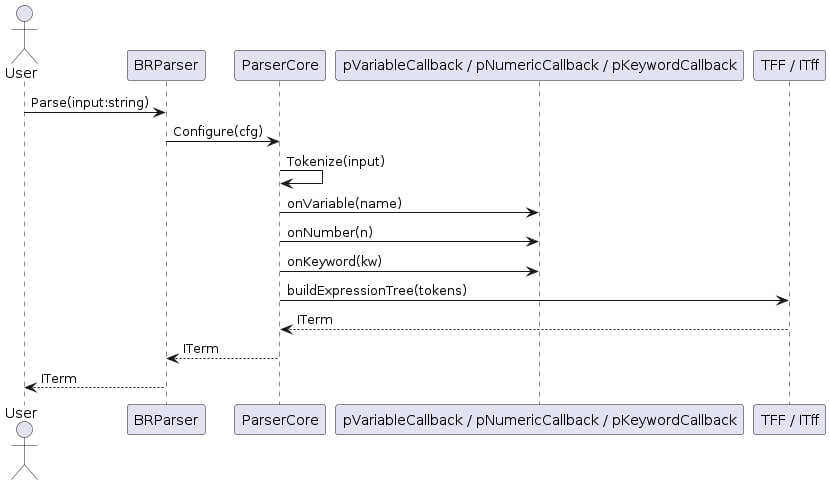
\includegraphics[width=0.9\textwidth]{./img/image.png}
  \caption{Временная диаграмма разбора выражения: взаимодействие User → BRParser → ParserCore → колбэки → TFF/ITff}
  \label{fig:parser-sequence}
\end{figure}

\begin{enumerate}
  \item \textbf{Разбор выражения:} 
    \[
      \texttt{let term = BRParser().Parse("\textbackslash x -> x x")}
    \]
    — библиотека выполняет конфигурацию (\texttt{Configure(cfg)}), токенизацию, вызывает последовательно колбэки \texttt{onVariable}, \texttt{onNumber}, \texttt{onKeyword}, затем строит AST с помощью переданных \texttt{TFF}/\texttt{ITff} и возвращает результат в виде \texttt{ITerm}. См. рис.~\ref{fig:parser-sequence}.

  \item \textbf{Пошаговая редукция:} 
    \[
      \texttt{let state = BetaReductor(cfg).EvaluateCode(code, true)}
    \]
    — выполняется один шаг бета‑редукции и возвращается новое состояние машины с обновлённым термом в регистре.

  \item \textbf{Полная нормализация:} 
    \[
      \texttt{BetaReductor(cfg).EvaluateCode(code, false)}
    \]
    — машина рекурсивно применяет \texttt{evaluateOneStep} до тех пор, пока термин не стабилизируется, и возвращает состояние с признаком \texttt{IsFinal = true}.
\end{enumerate}


\section{Ключевые фрагменты кода}

\subsection{Настройка парсера}
Комбинаторный подход на FParsec: конфигурация операторов и колбэков вынесена в отдельный блок.

\begin{lstlisting}[
  float=tb,frame=lines,
  label=lst:parser-config,
  caption=Конфигурация BRParser: операторы, ключевые слова и колбэки
]
// определить унарные и бинарные операторы с приоритетами
let brUnOps = [ UnOp {| keyword = "-"; term = atomicUnOpMinus; priority = 1 |} ]
let brBinOps = [
  BinOp {| keyword = "+"; term = atomicBinOpPlus;   priority = 1; 
        associativity = Associativity.Left |}
  BinOp {| keyword = "*"; term = atomicBinOpMult;   priority = 2; 
        associativity = Associativity.Left |}
  // ...
]

// объединить в конфиг
let cfg = {
  applicationTff     = appTff
  simpleLambdaTff    = SimpleLambdaTff(subs)
  multiLambdaTff     = Some (MultiLambdaTff(subs))
  operators          = brUnOps @ brBinOps
  keywords           = ["true"; "false"; "Y"; "NULL"]
  parseNumericConsts = true
  ifStatements       = false
}

// привязать колбэки для переменных, чисел, ключевых слов
p.pVariableCallback <- fun name -> DefaultVariable(name) :> ITerm
p.pNumericCallback  <- fun n    -> match n with Int i -> Data.Int i | 
    Float f -> Data.Float f
p.pKeywordCallback  <- function
  | "true"  -> Data.Bool true
  | "false" -> Data.Bool false
  | kw      -> raise (BRParsingException ...)
\end{lstlisting}

Пример задания конфигурации BRParser представлен в листинге \ref{lst:parser-config}.

\subsection{Механизм одного шага редукции}
Внутри \texttt{BetaReductor} ключевая функция \texttt{step} обрабатывает:
\begin{itemize}
  \item \textbf{β-редексы:} $(\lambda x.M)\,N \to M[x:=N]$;
  \item \textbf{спуск внутрь:} если редексов нет, рекурсивно обходит подтермы;
  \item \textbf{атомарные функции:} вызывает \texttt{IFunction.ReduceWithArguments}.
\end{itemize}

\begin{lstlisting}[
  float=tb,frame=lines,
  label=lst:machine-step,
  caption=Алгоритм одного шага в BetaReductor
]
let rec step term =
  match term with
  | :? IApplicationTerm as app ->
      match app.Function with
      | :? SimpleLambda as lam ->
          // бета-редукция: подстановка первого аргумента
          let arg = Seq.head app.Arguments
          substitution.Substitute(lam.Body, seq { lam.Variable, arg })
      | f when f :? IFunction ->
          // атомарный вызов
          f.ReduceWithArguments(app.Arguments, tff)
      | _ ->
          // спуск внутрь
          // 1) пытаемся step(f)
          // 2) если не изменилось, пробуем step на каждом аргументе
          term
  | :? IFunctionalAbstraction as lam ->
      // спуск внутрь тела λ
      let body' = step lam.GetBody
      if not (obj.ReferenceEquals(body', lam.GetBody)) then
        // пересоздать лямбду с новым телом
        SimpleLambda(lam.GetBoundVariable, body', substitution) :> ITerm
      else term
  | _ -> term
\end{lstlisting}

Алгоритм шага редукции представлен в листинге \ref{lst:machine-step}.

\section{Разработка тестовых примеров}
\label{sec:test-examples}

Для обеспечения надёжности и корректности работы как парсера, так и абстрактной машины бета‑редукции, был разработан обширный набор NUnit‑тестов.

\subsection{Тесты парсера}

Нижеследующие аспекты разбора покрываются тестами из модуля \texttt{ParseTest}:

\begin{itemize}
  \item \textbf{Лямбда‑абстракции:} проверяется, что строка вида \verb|\ x -> x| корректно преобразуется в \texttt{SimpleLambda}.  
  \item \textbf{Унарные и бинарные операторы:} приоритеты и ассоциативность обрабатываются в соответствии с конфигурацией \texttt{unOps} и \texttt{binOps}.  
  \\
  \item \textbf{Вложенные абстракции и приложения:} тестируются случаи \(\lambda x.\,\lambda y.\,\lambda z.\,y\) и \((\lambda x.\,x+x)\,5\).  
  \item \textbf{Скобочные конструкции:} проверяется различие между \(\,x + x - x\) и \(\,x + (x - x)\).  
  \item \textbf{Ключевые слова:} пользовательские ключевики (\texttt{magicWord0}, \texttt{magicWord1}) обрабатываются через колбэк \texttt{pKeywordCallback}.  
\end{itemize}

\begin{lstlisting}[float=tb,frame=lines,label=lst:parser-test-example,caption={Пример теста для скобочных выражений}]
[<Test>]
member this.Parentheses() =
  let noPar = "\\ x -> x plus x - x"
  let withPar = "\\ x -> x plus (x - x)"
  let gotNo = callParse2String(parser, noPar)
  let gotPar = callParse2String(parser, withPar)
  Assert.That(gotNo, Is.EqualTo(expectedNo))
  Assert.That(gotPar, Is.EqualTo(expectedPar))
\end{lstlisting}

Пример теста для скобочных выражений представлен в листинге \ref{lst:parser-test-example}.

\subsection{Тесты бета‑редуктора}

Тестовый модуль \texttt{BetaReductionTests} проверяет корректность шаговой и полной редукции:

\begin{itemize}
  \item \textbf{Один шаг vs. полная нормализация:} для терма \((\lambda x.\,x\,x)\,x\) сравнивается результат одного шага и финальной формы.  
  \item \textbf{Последовательность шагов:} функция \texttt{reduceStepByStep} строит весь путь редукции, и каждый промежуточный результат сравнивается с ожидаемым списком строковых представлений термов.  
  \item \textbf{Атомарные операции:} проверка встроенных бинарных операций, например \((+\,1\,2)\to 3\).  
  \item \textbf{Композиция λ‑выражений:} тесты для вложенных абстракций, например \(((\lambda x.\,x)\,(\lambda x.\,x))\) приводят к корректному результату.  
\end{itemize}

\begin{lstlisting}[float=tb,frame=lines,label=lst:reductor-step-test,caption={Проверка последовательности шагов редукции}]
[<Test>]
member _.``step by step plus``() =
  let plus = Data.BinOp("+", fun a b -> match a,b with Int x,Int y -> 
        Int(x+y) | _ -> failwith "")
  let term = applicationTff.CreateTerm([ plus; Data.Int 1; Data.Int 2 ])
  let seq = reduceStepByStep reductor (term2Code term)
  Assert.That(seq |> List.last, Is.EqualTo("Int 3"))
\end{lstlisting}

Проверка последовательности шагов редукции представлена в листинге \ref{lst:reductor-step-test}.

\section{Сравнение с существующими аналогами}
\label{sec:comparison-analogs}

Было произведено сравнение разработанного в данной работе решения с одним из аналогов визуализации работы абстрактной машины \textbf{WinCam} (см. рис.~\ref{fig:wincam}).


\subsection*{Преимущества WinCam}
\begin{itemize}
  \item Имеется визуализация термов в представлении де Брейна.
  \item Разработана встроенная справочная книга с набором готовых учебных примеров.
  \item Поддерживается выбор учебного языка из фиксированного набора.
\end{itemize}

\subsection*{Недостатки WinCam}
\begin{itemize}
  \item Интерфейс устаревший, перегруженный и плохо адаптирован под начинающих пользователей.
  \item Отсутствует модульность — невозможно добавить собственные вычислительные стратегии, лексемы или атомики без изменения исходного кода.
  \item Программа работает только под Windows и основана на устаревшем .NET Framework, что делает её недоступной для пользователей Linux и macOS.
\end{itemize}

\subsection*{Преимущества разработанного решения}
\begin{itemize}
  \item Реализована архитектура, ориентированная на расширяемость: пользователи могут определять собственные атомики (\texttt{IAtomic}), языковые конструкции \\(\texttt{ILanguageParser}) и стратегии редукции.
  \item Предусмотрена возможность свободного переключения между абстрактными машинами.
  \item Приложение сопровождается справочником с примерами, документацией и шаблонами использования.
  \item Кроссплатформенность — работает на Windows, Linux и macOS благодаря использованию .NET 8.0+.
\end{itemize}

\begin{figure}[h]
  \centering
  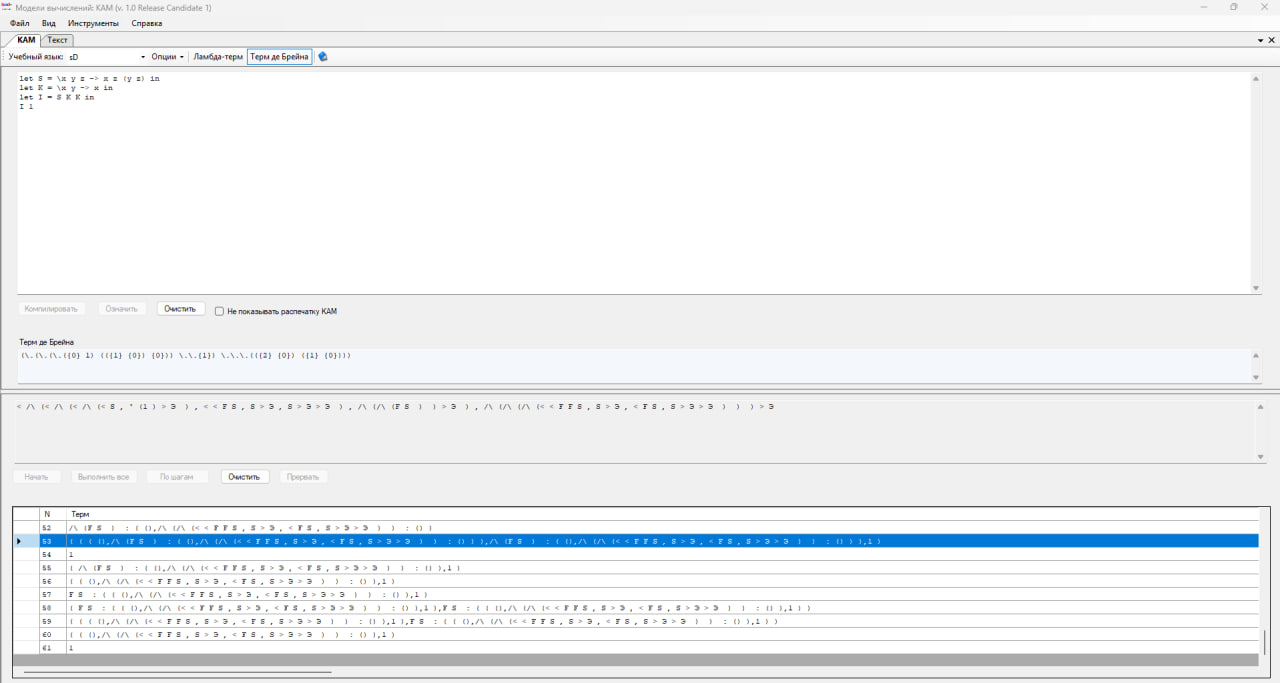
\includegraphics[width=0.8\textwidth]{./img/WinCam.png}
  \caption{Интерфейс WinCam: лямбда‑терм, отображение терма де Брейна и шаги КАМ}
  \label{fig:wincam}
\end{figure}

Графический пользовательский интерфейс WinCam представлен на рис. \ref{fig:wincam}.



\section{Выводы}
По итогам данной главы были достигнуты следующие результаты:
\begin{itemize}
  \item Представлена реализация бета-редуктора на платформе .NET с использованием языка F\# и библиотеки FParsec. Основное внимание было уделено структуре программного обеспечения, принципам модульности и расширяемости, ключевым компонентам (парсер, абстрактная машина, атомики) и механизмам настройки.
  \item Были разработаны сценарии использования системы — от разбора выражения до полной нормализации — и подтверждена корректность их реализации с помощью модульных тестов на базе NUnit. Предложенные подходы к конфигурации синтаксического анализатора и построению редуктора позволяют эффективно адаптировать систему под различные домены и языки.
  \item Сравнение с системой WinCam, показало, что разработанное решение обладает более современной архитектурой, кроссплатформенностью и гибкостью. Оно предоставляет пользователю расширенные возможности по настройке языка, визуализации и интеграции в другие проекты .NET.
\end{itemize}
Таким образом, реализованная система представляет собой современный, расширяемый и тестируемый инструмент для пошаговой редукции λ-термов, пригодный как для образовательных, так и для исследовательских целей.


\clearpage

\chapter*{Заключение}
\addcontentsline{toc}{chapter}{Заключение}

В заключении в тезисной форме необходимо отразить результаты работы:

\begin{itemize}
	\item аналитические (что изучено/проанализировано);
	\item теоретические;
	\item инженерные (что спроектировано);
	\item практические (что реализовано/внедрено).
\end{itemize}

Примерная формула такая: по каждому указанному пункту приводится по 3-5 результатов, каждый результат излагается в объеме до 5 фраз или предложений.

Также есть смысл привести предполагаемые направления для будущей работы.

Общий объем заключения не должен превышать 1,5 страниц (1 страницы для УИРов).

%%% Local Variables:
%%% TeX-engine: xetex
%%% eval: (setq-local TeX-master (concat "../" (seq-find (-cut string-match ".*-3-pz\.tex$" <>) (directory-files ".."))))
%%% End:


\label{end_of_main_text}

\setcounter{totalfigures}{\the\value{totalfigures}+\the\value{figure}}
\setcounter{figure}{0}
\setcounter{totaltables}{\the\value{totaltables}+\the\value{table}}
\setcounter{table}{0}
\setcounter{totallistings}{\the\value{totallistings}+\the\value{lstlisting}}
\setcounter{lstlisting}{0}

\makeatletter
\edef\@currentlabel{\the\value{totalfigures}}
\label{figures}
\edef\@currentlabel{\the\value{totaltables}}
\label{tables}
\edef\@currentlabel{\the\value{totallistings}}
\label{listings}
\makeatother

\clearpage

\phantomsection
\addcontentsline{toc}{chapter}{\bibname}	% Добавляем список литературы в оглавление
\printbibliography                        % печать библиографии через BibLaTeX

% \addcontentsline{toc}{section}{Список литературы}
% \begin{thebibliography}{99}


% \bibitem{Wolfengagen2004} {Ермаков А.Е.  Автоматизация онтологического инжиниринга в системах извлечения знаний из текста. М.: ООО ``ЭР СИ О'', Компьютерная лингвистика и интеллектуальные технологии: труды Международной конференци Диалог'2008, 2008.}


%\bibitem{Troel} {Троелсен Э. Язык программирования C\# 2008  и платформа .Net 3.5  М.: издательство <<Вильямс>>{}, 2010. 1344 с.}


%\bibitem{PBIRCH}{Ashwani Garg, Ashish Mangla, Neelima Gupta, Vasudha Bhatnagar PBIRCH: A scalable parallel clustering algorithm for incremental data. //Proceedings of 10th International Database Engineering and Applications Symposium IDEAS06, 2006}



% \end{thebibliography}

%%% Local Variables:
%%% TeX-engine: xetex
%%% eval: (setq-local TeX-master (concat "../" (seq-find (-cut string-match ".*-3-pz\.tex$" <>) (directory-files ".."))))
%%% End:


\endrefsection

\clearpage

%\chapter*{Приложения}
%\addcontentsline{toc}{chapter}{Приложения}
%\appendixtocon
%\renewcommand{\appendixname}{Приложение}
\appendix
\renewcommand{\thechapter}{\Asbuk{chapter}}
\renewcommand{\appendixtocname}{Приложения}
\addappheadtotoc
%\titleformat{\chapter}[block]{\centering\normalfont\Large\bfseries}{\chaptername{} \thechapter.}{1ex}{}{}
\renewcommand{\chaptername}{Приложение}
%\renewcommand*\printchaptername{\Large\bfseries\appendixname~}
%\renewcommand{\thechapter}{Приложение \Alph{chapter}}
%\renewcommand{\thechaptertoc}{Приложение \Alph{chapter}}

%\renewcommand{\chaptermark}[1]{\markboth{\chaptername\ \thechapter.\ #1}{}}

% \begin{appendices}

\chapter{Листинги основных структур разработанного модуля}\label{app-format}

\refsection

\lstinputlisting[
  label=lst:Lambda.fs,frame=lines,
  caption=Листинг из файла \texttt{Lambda.fs}
]{listings/Lambda.fs}

\lstinputlisting[
  label=lst:Atomic.fs,frame=lines,
  caption=Листинг из файла \texttt{Atomic.fs}
]{listings/Atomic.fs}

\lstinputlisting[
  label=lst:Environment.fs,frame=lines,
  caption=Листинг из файла \texttt{Environment.fs}
]{listings/Environment.fs}

\lstinputlisting[
  label=lst:Parser.fs,frame=lines,
  caption=Листинг из файла \texttt{Parser.fs}
]{listings/Parser.fs}

\lstinputlisting[
  label=lst:Machine.fs,frame=lines,
  caption=Листинг из файла \texttt{Machine.fs}
]{listings/Machine.fs}

\endrefsection

%%% Local Variables:
%%% TeX-engine: xetex
%%% eval: (setq-local TeX-master (concat "../" (seq-find (-cut string-match ".*-3-pz\.tex$" <>) (directory-files ".."))))
%%% End:

\clearpage

\chapter{Общая структура пояснительной записки}\label{app-structure}
%\addcontentsline{toc}{chapter}{}

\refsection

\begin{enumerate}
	\item Титульный лист %(в данном примере используется титульный лист от преддипломной практики)
	\item Лист с подписями (только для ВКР)
	\item Задание (в данном примере используется задание на диплом)
	\item Отчет из Антиплагиага \footnote{Обычно, допускается до 30\% заимствованного текста для работ бакалавров и до 20\% -- для работ магистров; см. соответствующие нормативные документы}
	\item Реферат (всегда на отдельной стр.)%, и эта страница \textit{НЕ} нумеруется)
	\item Оглавление. Начинается с новой страницы. %Обычно, это первая нумеруемая страница.
	\item Введение
	\begin{enumerate}
		\item Актуальность
		\item Новизна
		\item Оригинальная суть исследования
		\item Содержание ПЗ по главам (тезисно)
	\end{enumerate}
	\item Аналитическая глава. Пишется в стиле \textit{аналитического обзора}
	\item Теоретическая и инженерная глава. Описываются использованные, доработанные и разработанные модели, алгоритмы, методы, и т.п. Кроме того, тут формулируется архитектура системы.
	\item Инженерная глава. В этой главе следует отразить результаты проектирования, что, в общем случае, включает в себя следующие пункты:
	\begin{enumerate}
		\item Описание используемой методики проектирования
		\item Общая архитектура системы
		\item Архитектура подсистемы [таких подразделов может быть несколько штук, по одному на каждую подсистему или модуль, требующую детальное рассмотрение]
		\item Проектирование внешних и внутренних интерфейсов/протоколов взаимодействия
	\end{enumerate}
	\item Практическая глава. Описывается реализация, включая выбор инструментальных средств \footnote{В тех случаях, когда \begin{inparaenum}[(a)]\item этот выбор имеет существенное значение для всей работы и \item он не был, по каким-либо причинам, проделан в аналитической главе \end{inparaenum}}. Типовое содержание:
	\begin{enumerate}
		\item Состав и структура реализованного ПО 
		\item Выбор инструментальных средств
		\item Основные сценарии работы различных категорий пользователей
		\item Результаты тестирования (разработка тестовых примеров, таблицы и графики результатов прогона)
		\item Сравнение с существующими аналогами
	\end{enumerate}
	\item Заключение
	\item Список литературы 
	\item Приложения
\end{enumerate}

Кроме того, в ПЗ могут включаться и такие разделы, как словарь терминов, 
список сокращений и др. В зависимости от предпочтений автора, могут 
помещаться как в начале ПЗ (до оглавления), так и в конце (после заключения, 
но до приложений).

\paragraph{Замечания}: \mynobreakpar %\nopagebreak

\begin{enumerate}

  \item На каждый элемент из списка литературы должна быть хотя
бы одна ссылка в тексте.

  \item Список литературы должен быть оформлена согласно ГОСТ
\cite{Gost.7.1.2003,Gost.7.0.5.2008}.

  \item Минимальное количество источников для УИРов --- 15--20 (для
работ с большой аналитической и теоретической частью нормальное количество ---
25-30 и более), для дипломов --- соответственно, 30--35 и 35--60. Эти цифры
существенны, т.к. <<недобор>>, как правило, свидетельствует о не выполнении
аналитической части работы и, следовательно, недостаточном владении предметом.

  \item При подготовке РСПЗ рекомендуется вставлять уже наработанные к 
моменту подготовки РСПЗ материалы. Однако, в любом случае, каждый раздел 
должен начинаться с аннотации, заключенной в окружение \verb|\annotation|. В 
пояснительной записке к диплому аннотации не нужны. 

  \item Между заголовком главы и первым разделом рекомендуется поместить один-два абзаца связанного текста с кратким содержанием (планом) главы.

  \item Общее число и объем приложений не ограничивается. Объем ПЗ
\textbf{\textit{без}} приложений --- 25--40 стр. для УИРов, и не менее 60--100
стр. для дипломов. Объем ПЗ не может быть меньше указанных размеров. Это
означает, что студент не выполнил работу, или, как минимум, не удосужился
подготовить адекватную ПЗ. Превышать верхние пределы также не желательно, в
некоторых комиссиях это может восприниматься негативно; однако, в целом,
небольшое превышение допустимо, если проделана действительно большая работа и
получено много результатов (например, экспериментальных, или получены
нетривиальные аналитические или теоретические результаты).

  \item ГОСТ требует, чтобы нумерация страниц начиналась с 
первой, титульной, страницы. При этом на самой титульной странице номер не 
печатается. В данном случае, номера также не проставляются на листах задания, 
а также на листе с подписями (для ВКР).

\end{enumerate}

\printbibliography[heading=subbibliography]

\endrefsection

%%% Local Variables:
%%% TeX-engine: xetex
%%% eval: (setq-local TeX-master (concat "../" (seq-find (-cut string-match ".*-3-pz\.tex$" <>) (directory-files ".."))))
%%% End:


\clearpage

% \chapter{Правила использования шаблона}\label{app-manual}

Настоящий шаблон все еще несколько несовершенен в плане оформления: например, неправильная нумерация приложений, и еще несколько нюансов. В последующих версиях это будет исправляться.

Ниже описана структура исходных текстов шаблона (и, соответственно, структура исходных текстов ПЗ).

Кодировка всех файлов — UTF8, и для сборки PDF документов следует использовать
команду \texttt{xelatex}. При этом при работе через Sublime Text + LaTeXTools
следует использовтаь вариант сборщика Basic Builder.

В репозитории несколько <<головных>> файлов, предназначенных для генерации
документов на разных стадиях выполнения проекта.
\begin{itemize}
  \item[] \texttt{<проект>-1-task.tex} --- для генерации бланка задания;
  \item[] \texttt{<проект>-2-rspz.tex} --- для генерации отчета с титульным
  листом для РСПЗ;
  \item[] \texttt{<проект>-3-pz.tex} --- для генерации отчета с титульными
  листами для ПЗ.
\end{itemize}

Задача головных файлов --- <<склеить>> вместе разные части ПЗ. Каждая часть (реферат, введение, каждая содержательная глава, заключение, библиография, приложения) выделяется в отдельный файл. 

\begin{itemize}
  \item[] \texttt{thesis-abstract.tex} --- содержит аннотацию;
  \item[] \texttt{thesis-intro.tex} --- содержит введение;
  \item[] \texttt{thesis-chapter1.tex} --- текст первой главы;
  \item[] \texttt{thesis-chapter2.tex} --- текст второй главы;
  \item[] \texttt{thesis-chapter3.tex} --- текст третьей главы;
  \item[] \texttt{thesis-bibl.tex} --- список литературы (только подключение к
  проекту);
  \item[] \texttt{biblio.bib} --- собственно библиография (в формате BibTeX);
  \item[] \texttt{thesis-conclusion.tex} --- заключение;
  \item[] \texttt{thesis-appendix1.tex} --- первое приложение;
  \item[] \texttt{thesis-appendix2.tex} --- второе приложение;
\end{itemize}

Другие файлы, используемые для настройки шаблона и определения параметров
проекта:

\begin{itemize}
  \item[] \texttt{thesis-macro.tex} --- содержит определения различных
  макрокоманд, которые часто используются в конкретной работе, например,
  определения окружения для теорем, некоторые часто используемые формулы, и
  т.~п.;
  \item[] \texttt{0-0-project-members.tex} --- информация о проекте:
  руководитель, студент, тема и т. п.;
  \item[] \texttt{0-1-task-data.tex} --- информация о задании;
  \item[] \texttt{\_content.tex} --- склеенное основное содержимое отчета,
  которое используется для генерации ПЗ и РСПЗ;
\end{itemize}

%Одна из первых вещей, которые необходимо сделать при использовании данного шаблона --- это отредактировать аргумент команды \verb|\headertext| в начале головного файла.

Головные файлы следует менять только в том случае, если требуется сгенерировать
документ, изначально не предусмотренный в данном шаблоне. Если требуется
добавить новые файлы к основному содержимому проектка — новый раздел отчета или
приложения, следует вносить изменения в \texttt{\_content.tex}.

\section{Титульные листы}

Существует два варианта генерации титульных листов:

\begin{itemize}
  \item использование листов, сверстанных в \LaTeX{} (используется по
  умолчанию);
  \item подстановка пустых бланков из PDF-файлов.
\end{itemize}

\subsection{Титульные листы LaTeX}

Проект содержит определения титульных листов, описанные в виде \textbf{.tex}
файлов. На данный момент требуется заполнение данных студента вручную. Позже
будет реализована автоматическая подстановка данных проекта при инициализации
репозитория.

\subsection{Титульные листы из PDF}

При возникновении проблем с использованием титульных листов \LaTeX{} возмодно
включить в документ бланки титульных листов из PDF-файлов. Для этого нужно
раскомментировать соответствующие команды \textbf{includepdf} в начале
документа.

Для того, чтобы \LaTeX{} при компиляции автоматически <<подхватил>> задание, его
нужно сохранить в формате pdf (например, с помощью вирутального принтера),
поместить в ту же папку \texttt{/title} и назвать \texttt{task.pdf}. Точно также
следует поступить с титульной страницей (\texttt{title.pdf}). При оформлении ПЗ
для ВКР следует дополнительно поместить в папку \texttt{/title} pdf-версию листа
с подписями, назвав файл \texttt{title-dep22.pdf}. После этого нужно
раскомментировать команду
\begin{center}
  \verb|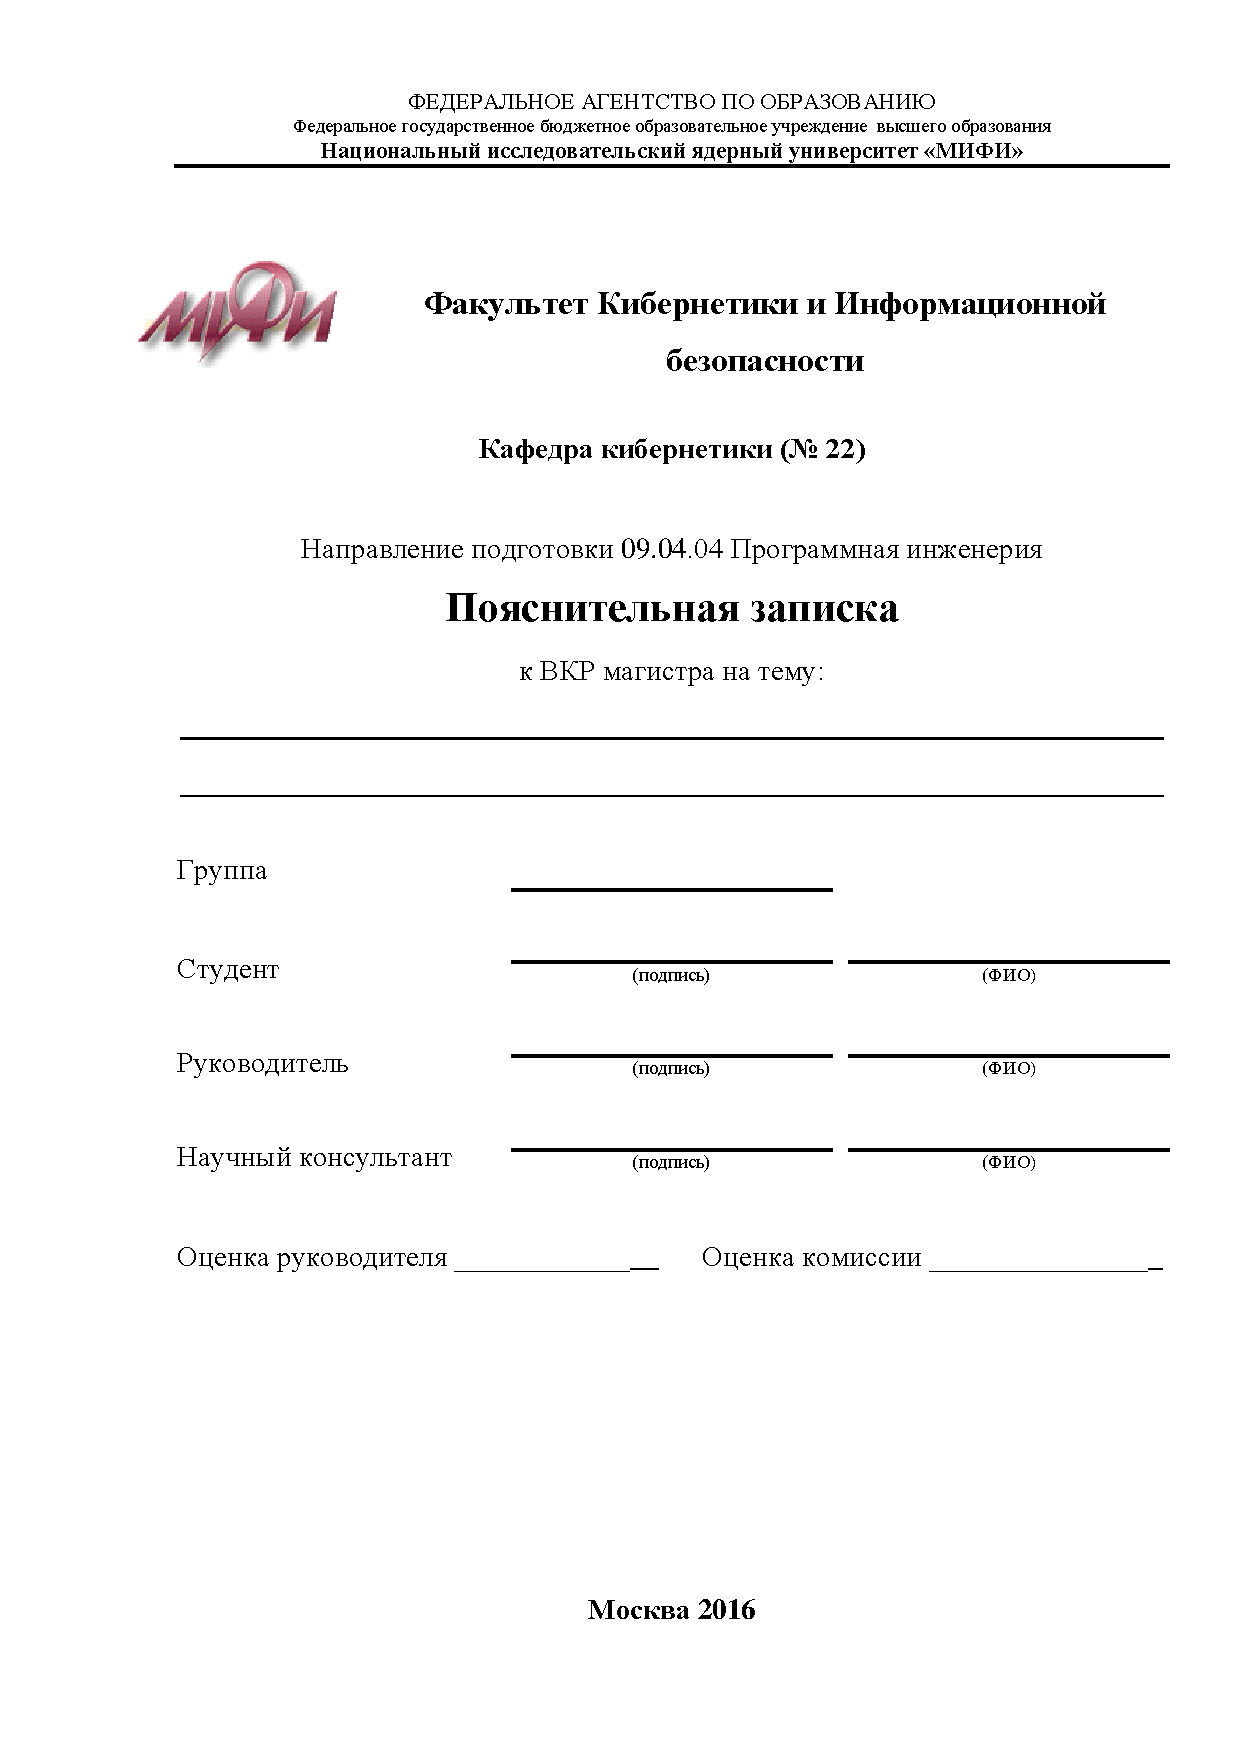
\includepdf[ ... ]{title/title-dep22.pdf}|
\end{center}
в начале головного файла.

Образцы и Word-шаблоны титульных листов для (РС)ПЗ к УИРам, НИРам, практикам и
ВКР доступны в репозитории
\begin{center}
  \url{https://gitlab.com/skibcsit/thesis-titles}.
\end{center}  

\textbf{Замечание}. В шаблоне используется пакет \texttt{hyperref}, который
делает две вещи: все перекрестные ссылки <<кликабельны>>, а также выделены
(красной) рамочкой. Эти рамки \textit{не выводятся на печать}. Вместо цветных
рамок, возможны другие способы выделения ссылок (см. документацию пакета).

%%% Local Variables:
%%% TeX-engine: xetex
%%% eval: (setq-local TeX-master (concat "../" (seq-find (-cut string-match ".*-3-pz\.tex$" <>) (directory-files ".."))))
%%% End:


% \end{appendices}

\label{end_of_document}

%%% Local Variables:
%%% TeX-engine: xetex
%%% eval: (setq-local TeX-master (concat "../" (seq-find (-cut string-match ".*-3-pz\.tex$" <>) (directory-files ".."))))
%%% End:
